\reportheading{2.\quad Methodology}
Fire Dynamics Simulator (FDS) version 6.10.1 was used for both tasks~\cite{fdsuser}. The propane runs reproduce the conditions of the ceiling-temperature experiment. The propylene runs include soot production, ceiling extraction and make-up air so that the available clear height can be assessed.

\reportfigure{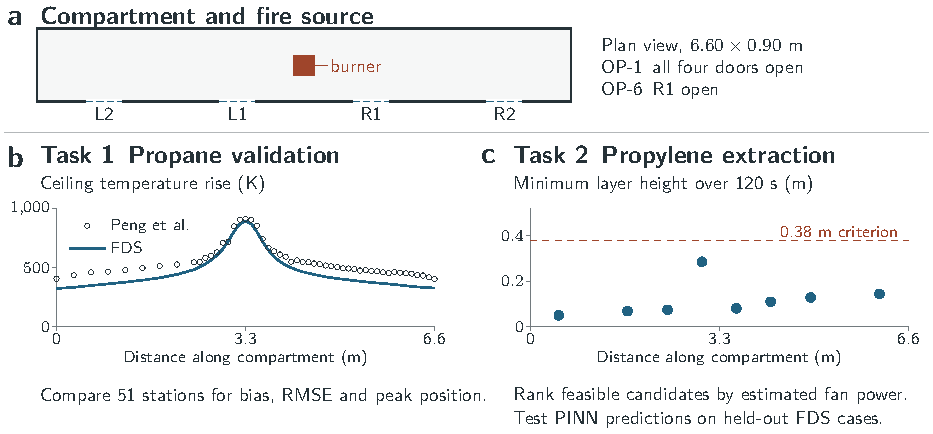
\includegraphics[width=.98\linewidth]{figures/study-workflow.pdf}}{Query order for Bayesian optimisation (BO) and the genetic algorithm (GA, seed 0). Rows increase in curtain depth and columns in flow. Teal marks the largest clearance margin in the archived set.}


\subhead{2.1\quad Task 1 --- Propane fire and ceiling-jet validation}
The geometry follows Fig.~1 of the Topic B brief and the compartment tested by Peng et al.~\cite{peng}. The compartment measured $6.60 \times 0.90 \times 0.76$~m internally, with a 0.25~m square burner on the floor at $x=3.30$~m. Along one side wall, the openings were L2, L1, R1 and R2 in order of increasing $x$. Each was 0.43~m wide and 0.63~m high. The domain extended outside this wall to $y=1.40$~m so that air could enter at one height and leave through the same door at another. The reference ambient temperature was $27.5\,^{\circ}$C.

Group~18 used both nominal fire powers, 47.2 and 106.2~kW, under each door state, OP-1 with all four doors open and OP-6 with only R1 open. FDS specifies heat release per unit burner area. Since the burner edges follow the mesh faces, we checked the resulting burner area on each grid together with the heat release rate recorded during the run.

\clearpage
\subhead{Spatial resolution and physical submodels}
The OP-1 study used $132\times28\times19$, $176\times36\times25$ and $220\times48\times32$ cells over the same domain. Following the FDS User’s Guide~\cite{fdsuser}, the characteristic fire diameter was calculated as
\[
 D^*=\left(\frac{\dot Q}{\rho_\infty c_p T_\infty\sqrt{g}}\right)^{2/5}.
\]
Here $\dot Q$ is the nominal fire power and $g$ is gravitational acceleration. The ambient air properties are density $\rho_\infty$, specific heat $c_p$ and absolute temperature $T_\infty$. Dividing $D^*$ by the longest cell dimension gives a common measure of resolution. The change in the longitudinal temperature profile shows what that resolution means for the result.

\subhead{Task 1 --- Controlled comparisons and experimental measurements}
For OP-1 at 106.2~kW, we first held the coarse grid and radiative fraction (0.29) fixed and changed the subgrid closure from Deardorff to WALE~\cite{fdstech}. Yuen et al.\ also compared closures for compartment fires~\cite{yuen}. We then retained Deardorff and set the radiative fraction to 0.20 and 0.50 in separate runs. A further comparison replaced the adiabatic lining with a conducting board. The experiment supplied the board thickness of 15~mm. The FDS Steckler insulation example supplied proxy values for density (200~kg/m$^3$), conductivity (0.10~W/(m\,K)) and specific heat (1.0~kJ/(kg\,K))~\cite{steckler}. Both wall conditions used the $154\times56\times23$ doorway grid for OP-6 and the original coarse grid for OP-1 at 47.2~kW.

Figure~9 of Peng et al.~\cite{peng} gives the measured ceiling-temperature rise along the compartment. We digitised 51 positions on each profile and paired them with readings from modelled 1~mm thermocouples at $z=0.74$~m. At position $i$, the FDS rise is the mean temperature over 90--120~s, weighted by the actual device intervals, less the model ambient temperature. With $e_i=\Delta T_{\mathrm{FDS},i}-\Delta T_{\mathrm{exp},i}$, the mean bias and root mean square error are
\[
 \mathrm{bias}=\frac{1}{51}\sum_{i=1}^{51}e_i,\qquad
 \mathrm{RMSE}=\sqrt{\frac{1}{51}\sum_{i=1}^{51}e_i^2}.
\]
The distance from the burner to the hottest station gives a separate measure of peak displacement. Over the same interval, the R1 profiles show which part of the door admitted cool air and which part carried hot gas out. The wall and radiation comparisons examine how heat loss also affects the ceiling temperature.

\subhead{Compartment plan and extraction layout}
\begingroup\centering
\setlength{\unitlength}{0.88pt}
\begin{picture}(420,104)
\put(24,28){\framebox(363,49.5){}}
\put(24,76){\line(1,0){363}}
\linethickness{2pt}
\multiput(57.55,77.5)(90.75,0){4}{\line(1,0){23.65}}
\linethickness{0.4pt}
\put(69,85){\makebox(0,0){L2}}
\put(160,85){\makebox(0,0){L1}}
\put(251,85){\makebox(0,0){R1}}
\put(342,85){\makebox(0,0){R2}}
\put(178,28){\line(0,1){49.5}}
\put(233,28){\line(0,1){49.5}}
\put(183.5,30.75){\framebox(22,44){}}
\put(205.5,30.75){\framebox(22,44){}}
\put(198.625,45.875){\dashbox{1.25}(13.75,13.75){}}
\linethickness{2pt}
\put(24,28){\line(0,1){49.5}}
\put(387,28){\line(0,1){49.5}}
\linethickness{0.4pt}
\put(24,18){\line(1,0){363}}
\put(24,15){\line(0,1){6}}
\put(387,15){\line(0,1){6}}
\put(205,8){\makebox(0,0){6.60 m}}
\end{picture}\par
\endgroup
\tablenote{Plan view of the nominal inputs. The long wall carries the four labelled doorways. In the paired-flow design, the heavy end lines mark make-up openings, the two full-width interior lines mark curtains and the adjoining rectangles mark ceiling exhausts. The dashed square marks the floor burner under the exhausts. The end openings, curtains and exhausts apply to Task~2.}


\clearpage
\subhead{2.2\quad Task 2 --- Propylene fire and smoke extraction design}
For the nominal 106.2~kW propylene fire, the baseline soot yield was 0.02~kg/kg of fuel and the CO yield was 0.01~kg/kg. Additional runs raised the soot yield to 0.05 and 0.10~kg/kg while retaining the same CO yield. Each of the three soot yields was tested with OP-1 and OP-6, giving six scenarios with the doors held in position throughout each fire. The original design grid had $132\times28\times19$ cells and adiabatic enclosure surfaces.

\subhead{Candidate screening and design changes}
The archived FDS results support two comparisons of checking order. For the original layout, the next choice was a design. For the revised layout, the choice was which of six scenarios to check first at a given flow. We also examined the effect of changing the flow order.

An initial OP-6 screen at baseline soot yield crossed four curtain depths (0, 0.08, 0.16 and 0.24~m) with four total exhaust flows (0.08, 0.16, 0.24 and 0.32~m$^3$/s). The fixed-order benchmark, Bayesian optimisation (BO)~\cite{bo} and a genetic algorithm (GA)~\cite{ga} began with the same four corner designs. Each query revealed one archived FDS margin. BO and GA used only the margins revealed so far to select their next design. We counted all queries through the first discovery of the largest recorded margin and repeated GA with 20 random seeds.

In the revised layout, replacement air enters at floor level through an opening in each end wall. The inlet height is 0.44~m with OP-1 and 0.48~m with OP-6. Above the burner, two ceiling vents each feed a separate exhaust branch. Transverse curtains at $x=2.8$ and 3.8~m extend 0.24~m below the ceiling on either side of the vents.

\reportfigure{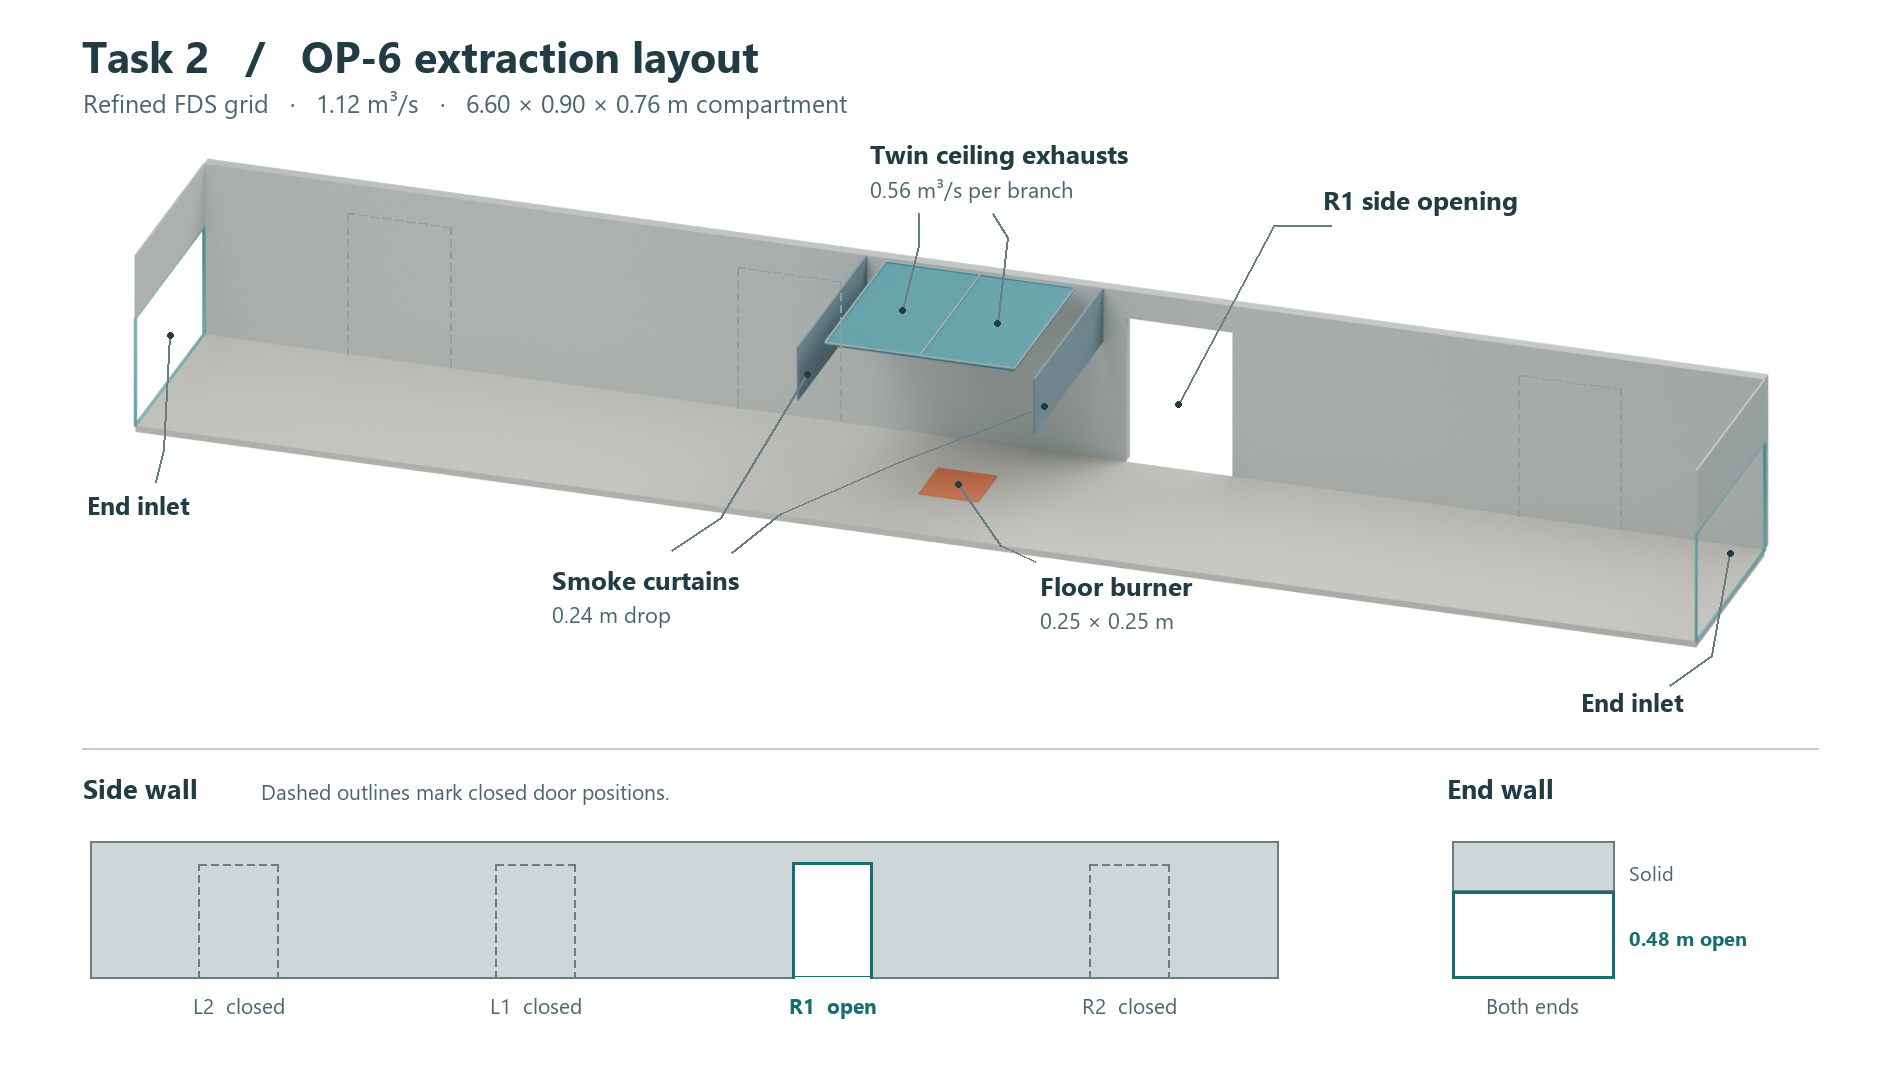
\includegraphics[width=\linewidth]{../figures/op6_1p12_fds_geometry_review.png}}{Cutaway of the refined OP-6 layout. The near wall is omitted from the view. In FDS it is a continuous adiabatic wall at $y=0$. R1 is the only open side door. Dashed outlines mark the three closed door positions. Both end walls admit make-up air through openings extending 0.48~m above the floor.}

With the two branches sharing the flow equally, we compared 0.96 and 1.28~m$^3$/s across all six scenarios. The refined grid also included the intermediate flow of 1.12~m$^3$/s. For the separate ranking study, we excluded both revised inlet families from training and retained increasing power order for the three flows. At each flow the physics-informed neural network (PINN)~\cite{pinn}, direct regression and their equal-weight average ranked the six scenarios from lowest to highest predicted clearance (Section~5.2).

\subhead{Layer-height criterion and local smoke measurements}
FDS reported a thermally inferred layer height $h_j(t)$ along eight vertical columns on the centreplane, $y=0.45$~m. Their longitudinal positions were 0.5, 1.7, 2.4, 3.0, 3.6, 4.2, 4.9 and 6.1~m. Devices were sampled nominally every 0.5~s. For scenario $s$ the sampled margin was
\[
 m_s=\min_{j,\,0\leq t\leq120\,\mathrm{s}} h_{j,s}(t)-0.38\,\mathrm{m}.
\]
Half the compartment height sets the clearance threshold. A single reading below it is sufficient to reject a candidate during screening. A candidate that clears this check needs a full 120~s record for each of the six scenarios. The smallest recorded margin then identifies the door state, soot yield, station and time governing the design. This check covers the eight instrumented columns.

\subhead{Task 2 --- Optical conditions, CO and fan power}
At the same stations, probes at $z=0.38$~m recorded visibility and CO volume fraction. A centreplane map of extinction shows how far smoke extends from the fire. These measurements describe local conditions at half height alongside the temperature-based clearance criterion. Fuel consumption and the specified yield determine the estimated mass of CO generated. The concentration at a probe also depends on how the gas travels, mixes with air and leaves the compartment. Recorded fire power was checked for each comparison.

For a total volume flow $Q$ divided equally between the two short exhaust branches, the estimated electrical input was
\[
 P_{\mathrm{el}}=\frac{Q\,\Delta p}{\eta},\qquad
 \Delta p=\left(f\frac{L}{D_h}+K\right)\frac{\rho}{2}
                 \left(\frac{Q}{2A}\right)^2 .
\]
Each short branch has area $A=0.32$~m$^2$, length $L=0.40$~m and assumed hydraulic diameter $D_h=0.533$~m. The loss calculation takes air density $\rho=1.2$~kg/m$^3$, Darcy friction factor $f=0.02$ and local loss coefficient $K=2$. The two branches run in parallel, so the same pressure drop applies to each. Applying fan efficiency $\eta=0.60$ to the combined flow gives the electrical input for these branches alone.

\subhead{Selection and verification of the design flow}
For the flow selection we doubled the vertical cell count from 19 to 38 and retained the horizontal grid, inlet settings and curtains. The intermediate setting of 1.12~m$^3$/s lies halfway between the original flows. Figure~4b compares all three on the refined grid for OP-6 at baseline soot yield. Table~D3 checks the selected flow against the eight station histories over 120~s for each combination of door state and soot yield.
\clearpage
\subhead{2.3\quad Constrained optimisation of the extraction system}
The brief specifies a minimum clear height and requires a power estimate for mechanical extraction. Group~18 chose minimum required fan input power as the design objective. Let $g$ denote a candidate layout, $Q$ the total extraction rate in m$^3$/s and $P$ the required electrical input in watts. We formulated the design problem as
\begin{equation}
\begin{aligned}
\min_{g,Q,P}\quad &P\\
\mathrm{s.t.}\quad
 &h_{s,i,t}(g,Q)\geq 0.38\,\mathrm{m}
       &&\forall s\in S,\ i\in I,\ t\in T_s,\\
 &P\geq Q\,\Delta p_s(g,Q)/\eta_s(g,Q)
       &&\forall s\in S,\\
 &g\in G,\quad Q\in\mathcal Q(g),\quad P\geq0 .
\end{aligned}
\label{eq:design}
\end{equation}
$G$ contains the candidate vent, curtain and make-up layouts. A door-dependent inlet preset is part of $g$. One setting is specified in advance for each door state and applies to all soot yields in that state. The same $Q$ is selected from the tested flows $\mathcal Q(g)$ for every scenario. The six members of $S$ combine the two door states with the three soot yields. $I$ contains the eight station positions, and $T_s$ contains the stored device times over the full 120~s run. The first constraint tests every recorded station and time. The second sizes electrical input for the largest required power across the scenarios, with pressure drop $\Delta p_s$ in Pa and total efficiency $0<\eta_s\leq1$.

For the two equal-flow branches, we evaluate power using the short-branch loss estimate in Section~2.2. Remaining ductwork and equipment losses are unknown. We evaluate feasibility by enumerating the tested candidates and computing the worst sampled clearance,
\[
m(g,Q)=\min_{s\in S,\ i\in I,\ t\in T_s}
           \{h_{s,i,t}(g,Q)-0.38\,\mathrm{m}\}.
\]
One negative margin excludes a design. A feasible design must have $m\geq0$ over the full set of records, after which its electrical input can be compared with that of other feasible designs. If every candidate falls short, the design with the largest margin provides a starting point for the next layout. The Bayesian and genetic searches in Section~5.2 are assessed on how soon they locate that design.
